\chapter{Manipulating Template Pixels for Model Adaptation of Siamese Visual Tracking}\label{chap:MTP}

\section{Abstract}
In this letter, we show that the challenging model adaptation task in visual object tracking can be handled by simply manipulating pixels of the template image in Siamese networks. For a target that is not included in the offline training set, a slight modification of the template image pixels will improve the prediction result of the offline trained Siamese network. The popular adversarial example generation methods can be used to perform template pixel manipulation for model adaptation. Different from current template update methods, which aim to combine the target features from previous frames, we focus on the initial adaptation using target ground-truth in the first frame. Our model adaptation method is pluggable, in the sense that it does not alter the overall architecture of its base tracker. To our knowledge, this work is the first attempt to directly manipulating template pixels for model adaptation in Siamese-based trackers. Extensive experiments on recent benchmarks demonstrate that our method achieves better performance than some other state-of-the-art trackers. Our code is available at https://github.com/lizhenbang56/MTP.

\section{Introduction}
Object tracking refers to the task of sequentially locating a specified moving object in a video, given only its initial state. Recently, Siamese networks \cite{danelljan2019atom, bertinetto2016fully} have demonstrated a significant improvement in object tracking performances. Siamese trackers formulate the visual object tracking problem as learning cross-correlation similarities between a target template and a search region. Tracking is then performed by finding the target object from the search image region by computing the highest visual similarity. Despite its recent success, the learned similarity measure of the Siamese network is not necessarily reliable for objects that are not included in the offline training set, leading to poor generalization \cite{Bhat_2019_ICCV}. Several recent works aim to adapt the model to the current target appearance. For example, TADT \cite{Li_2019_CVPR} identifies the importance of each convolutional filter according to the back-propagated gradients and selects the target-aware features based on activations for representing the targets. However, the feature extractor of TADT is pre-trained on ImageNet \cite{russakovsky2015imagenet}, not on large-scale visual tracking datasets. This limits the representation ability of its features on the object tracking task. GradNet \cite{Li_2019_ICCV} exploits the discriminative information in gradients and updates the template in the Siamese network through feed-forward and backward operations. However, the extra sub-network increases the computational cost and is prone to overfitting. UpdateNet \cite{Zhang_2019_ICCV} learns to combine the target features from previous frames. However, it does not use ground truth information to adaptively adjust the template features of the first frame.

\begin{figure}[t]
    \centering
    \includegraphics[width=0.48\textwidth]{Img/MTP/got10k/visulization2.pdf}
    \caption{A comparison of our method with the state-of-the-art trackers ATOM \cite{danelljan2019atom} and SiamFCv2 \cite{bertinetto2016fully} in challenging situations. The example frames are from the GOT-10k \cite{huang2018got} testing set.}
    %\caption{A comparison of our method with ATOM \cite{danelljan2019atom} and SiamFCv2 \cite{bertinetto2016fully}. The example frames are from the GOT-10k \cite{huang2018got} testing set.}
    \label{fig:vis}
\end{figure}

In this work, we show that the challenging model adaptation task in visual object tracking can be handled by simply manipulating pixels of the template image in Siamese networks. Given an object tracker, our algorithm modifies template pixels in only a few gradient-descent iterations using the target ground-truth in the first frame. For a target that is not included in the offline training set, we believe that a slight modification of the template image pixels can improve the prediction result of the offline trained Siamese network. We use the adversarial example generation method to achieve this, because it is commonly used to slightly modify the input image, and thereby impose an impact on the prediction result of the network. We depart from the purpose of adversarial sample generating in that the latter is aimed to make the prediction of the network worse, while we hope the prediction of the Siamese network is better. The proposed model adaptation method can be integrated with varieties of Siamese trackers like SiamFC++ \cite{SiamFC++}. Note that the parameters of the Siamese network remain intact to preserve the generative ability of offline-trained embedding space. We perform comprehensive experiments on 4 tracking benchmarks: VOT2018\cite{kristan2018sixth}, TrackingNet\cite{muller2018trackingnet}, GOT-10k\cite{huang2018got}, and OTB2015\cite{wu2013online}. Our approach achieves state-of-the-art results while running at over 80 FPS (see Fig. \ref{fig:vis}).

\section{Proposed Algorithm}
In this section, we present a new model adaptation approach for Siamese trackers via directly manipulating template pixels. We start by revisiting the tracking process of popular template matching-based trackers, which is closely related to the proposed approach. Following \cite{Danelljan_2020_CVPR}, we formulate object tracking as a confidence-based regression problem, which learns a function $s_\theta:\mathcal{Y\times X\rightarrow \mathbb R}$, and predicts a scalar confidence score $s_\theta(y,x)\in\mathbb R$ given an output-input pair $(y,x)$. The final estimate $f(x)=y^*$ is predicted as follows:
\begin{equation}
    f(x) = \arg\max_{y\in \mathcal Y}s_\theta (y,x),
\end{equation}
where $x$ is an input image. $y$ usually represents the center 2D image coordinate of the target object. Currently, there are two prevalent template matching-based paradigms: discriminative correlation filter (DCF) approaches and Siamese tracking methods.

In DCF-based methods, a circular correlation filter $w_{\theta}$ is trained during tracking to predict a target confidence score:
\begin{equation}
    s_\theta(y,x)=(w_\theta * \phi(x))(y),
    \label{equ:dcf}
\end{equation}
where $\phi(x)$ is the features extracted from the search image $x$.

In contrast to DCF, Siamese trackers exploit a two-stream architecture. One stream extracts the target’s features $\phi_\theta(z)$ based on the template image $z$ which is cropped from the first frame according to the ground truth bounding box. The other stream receives as input a large search image $x$ and outputs the search features $\phi_\theta(x)$. The two outputs are cross-correlated to predict a target confidence score:
\begin{equation}
    s_\theta(y,x)=(\phi_\theta(z) * \phi_\theta(x))(y).
    \label{equ:siamese}
\end{equation}

DCF-based trackers and Siamese trackers both have the advantage of utilizing large-scale visual tracking datasets to train the feature extractor $\phi(\cdot)$ or the embedding network $\phi_{\theta}(\cdot)$ by their own right. This way the representation ability of features on the object tracking task can be enhanced. 

In contrast to Siamese trackers, DCF learns the filter $w_\theta$ from example patches of the target appearance to discriminate it from the background.
Despite the improved tracking efficiency using the circular correlation operation, its boundary effect and sophisticated optimization prevent itself from making a good trade-off between computational speed and tracking performance. Siamese trackers do better in this aspect, although the learned similarity measure in the cross-correlation is not necessarily reliable for objects that are not included in the offline training set, leading to poor generalization.

In this letter, we aim to design a new Siamese tracking method that has the ability to make full use of the specific information of the current video for model adaptation like the DCF-based trackers, although the object in it is not included in the offline training set. This is achieved by utilizing the annotation information in the first frame to perform model adaptation.

Note that Equ. (\ref{equ:dcf}) and Equ. (\ref{equ:siamese}) bear some similarities with each other, and the main difference lies in the kernel term for correlation: the kernel of DCF is the online-learned $w_{\theta}$, and the kernel of the Siamese network is $\phi_\theta(z)$. In order for the Siamese network to have the model adaptation ability, we need to adapt $\phi_\theta(z)$ using the first frame ground truth annotation of the current video. There are two design choices to adapt $\phi_\theta(z)$: changing $\phi_\theta(\cdot)$ or changing $z$. However, changing $\phi_\theta(\cdot)$ may cause too much tedious meta-learning settings to ensure the generative ability of offline-trained embedding space \cite{ROAM, DBLP:conf/aaai/JungYNCH20}. In contrast, our solution is in a simple way to perform model adaptation of Siamese trackers by changing $z$, i.e., modifying template pixels in only a few gradient-descent iterations using the target ground-truth at the first frame. Compared with current model adaptation methods of Siamese trackers, the proposed method has the following advantages. First, we never modify parameters of the Siamese network to preserve the representation ability of offline-trained embedding space. Second, different from current template update methods \cite{zhu2018distractor, Zhang_2019_ICCV}, which aim to combine the target features from previous frames, we focus on the initial adaptation using target ground-truth at the first frame. Finally, our model adaptation method is pluggable, in the sense that it does not alter the overall architecture of the base tracker. In the next subsection, we will show how the popular adversarial example generation methods can be used to perform template pixel manipulation for model adaptation.

\subsection{Manipulating Template Pixels for Model Adaptation}
At first glance, there may be a contradiction between the model adaptation task and the adversarial example generation task, because these two tasks have different purposes. An adversarial example \cite{kurakin2017adversarial} is a sample of input data which has been modified very slightly in a way that is intended to perform an attack on machine learning systems, which means to cause a machine learning model to make wrong predictions. However, the purpose of model adaptation in our work is to make full use of the annotation information in the first frame to improve the tracking performance for the current video. We will point out in the following that there are some similarities between these two tasks and we can utilize adversarial example generation methods to perform the model adaptation task.

Before introducing the proposed method, we first revisit the popular adversarial example generation methods. One of the simplest methods to generate adversarial images $I^{adv}$ works by linearizing loss function in $L_{\infty}$ neighbourhood of a clean image and finds exact maximum of linearized function using following closed-form equation \cite{FGSM}:
\begin{equation}
    I^{adv} = I + \epsilon \text{ sign} \bigl( \nabla_I L(I, y_{true})  \bigr),
\end{equation}
where $I$ is the input image, and the values of the pixels are integer numbers in the range [0, 255]. $y_{true}$ is the true label for the image $I$. $L(I, y)$ is the cost function of the neural network for the attack purpose, given image $I$ and label $y$. $\epsilon$ is a hyper-parameter to be chosen. A straightforward way to extend the above method is applying it multiple times with small step size, and clipping pixel values of intermediate results after each step to ensure that they are in an $\epsilon$-neighbourhood of the original image.  This leads to the Basic Iterative Method (BIM) introduced in \cite{kurakin2017adversarial}: 
\begin{equation}
    \begin{gathered}
        I_0^{adv} = I, \\
        I_{N+1}^{adv} = Clip_{I,\epsilon}\{I_N^{adv}+\alpha \text{ sign}(\nabla_I L(I_N^{adv},y_{true}))\},
    \end{gathered}
\end{equation}
where $Clip_{I, \epsilon} \left\{ I' \right\}$ is the function which performs per-pixel clipping of the image $I'$, so that the result will be in $L_{\infty}$ $\epsilon$-neighbourhood of the source image $I$.
The BIM can be easily made into an attacker for a specific desired target class, called the Iterative Target Class Method \cite{kurakin2017adversarial}:
\begin{equation}
    \begin{gathered}
        I_0^{adv} = I,\\
        I_{N+1}^{adv} = Clip_{I,\epsilon}\{I_N^{adv}-\alpha \text{ sign}(\nabla_I L(I_N^{adv},y_{target}))\}.
    \end{gathered}
    \label{equ:itcm}
\end{equation}
Equ. (\ref{equ:itcm}) shows that manipulating pixels of the input image in only a few gradient-descent iterations is able to change the network's prediction to the target class $y_{target}$. Note that our purpose is manipulating pixels of the template image in the first frame, so that the prediction is closer to the ground truth bounding box. So we can perform model adaptation for Siamese networks using Equ. (\ref{equ:itcm}) with some modifications:
\begin{equation}
    \begin{gathered}
        z_0 = z,\\
        z_{N+1} = Clip_{z,\epsilon}\{z_N -\alpha \text{ sign}(\nabla_z L(z_N,y_{bb}))\},
    \end{gathered}
    \label{equ:adaptaion}
\end{equation}
where $z$ is the template image in the first frame, and $y_{bb}$ is the label for Siamese trackers generated from the ground truth bounding box. In the next subsection, we will introduce the overall tracking process equipped with the proposed model adaptation module.

%%%%%%%%%%%%%%%%
\begin{table}[t]
\renewcommand\arraystretch{0.8}
\caption{State-of-the-art comparison on the popular tracking benchmark OTB2015 with the running speed. FPS: frame per second. Our speed is tested on an NVIDIA RTX 2080Ti GPU.}
\setlength{\tabcolsep}{3pt}
\begin{center}
\begin{tabular}{l | c c c c c c}
\toprule
Trackers & ECO & MDNet & SiamRPN++ & ATOM & SiamFC++\_G & Ours \\
\midrule
Success & 70.0 & 67.8  & 69.6      & 66.9      & 68.3       & 69.7 \\
FPS     & 8    & 1     & 35        & 30       & 90         & 82  \\
\bottomrule
\end{tabular}
\end{center}
\label{table:otb}
\end{table}
%%%%%%%%%%%

%%%%%%%%%%%%%%%%
\begin{table}[t]
\renewcommand\arraystretch{0.8}
\centering
\caption{state-of-the-art comparison on the TrackingNet test dataset in terms of precision, normalized precision and success.}
\begin{tabular}{l c c c}
\toprule
Method   &  Prec.   &  Norm. Prec. & Succ.  \\
\midrule
Ours  &  70.6&  81.7 &74.9 \\
SiamFC++\_G& 70.5 & 80.0 & 75.4 \\
SiamFC++\_A  & 64.6 & 75.8 & 71.2 \\
ATOM              & 64.8 & 77.1 & 70.3 \\
SiamRPN++&  69.4 & 80.0 &73.3 \\
MDNet	 &  56.5&  70.5 &60.6 \\
ECO	 &  49.2&  61.8 &55.4 \\
SiamFC	 &  51.8&  65.2 &55.9 \\
\bottomrule
\end{tabular}
\label{tabel:trackingnet}
\end{table}
%%%%%%%%%%%

%%%%%%%%%%%%%%%%%
\begin{figure}[t]
    \centering
    \includegraphics[width=0.4\textwidth]{Img/MTP/got10k/success_plot.png}
    \caption{Comparing the results of our approach against other approaches over the GOT-10k test set. The trackers are ranked by their average overlap scores.}
    \label{fig:got10k}
\end{figure}
%%%%%%%%%%%%

%%%%%%%%%%%%%%%%%%%%%%%%%%%%%%%
\subsection{Tracking Framework}
The proposed model adaptation method is integrated with the SiamFC++ tracker \cite{SiamFC++} in a plug-and-play manner. SiamFC++ is based on SiamFC \cite{bertinetto2016fully} and progressively refined according to several guidelines proposed in \cite{SiamFC++}. The input of the original SiamFC++ network is composed of the template image $z_0$ cropped from the first frame and search image $x_i$ cropped from the $i$-th frame. However, we expect to perform template manipulating such that, after $N$ steps of pixel update on the input pair $(z_0, x_0)$ to obtain $z'$, the tracker performs well on $(z', x_i)$. To achieve this, we start by cropping the initial template image $z_0\in\mathbb R^{3\times128\times 128}$ and the initial search image $x_0\in\mathbb R^{3\times289\times 289}$ from the first frame using the ground truth bounding box.
Then, $z_0$ and $x_0$ are sent to the SiamFC++ network to obtain the tracking prediction of the first frame. The tracking loss in SiamFC++ \cite{SiamFC++} is calculated as follows:
\begin{equation}
    L = L_{\text{cls}} + L_{\text{quality}} + L_{\text{reg}},
\end{equation}
where $L_{\text{cls}}$ is the focal loss \cite{lin2017focal}. $L_{\text{quality}}$ is the binary cross entropy (BCE) loss for quality assessment. $L_{reg}$ is the IoU loss \cite{yu2016unitbox} for bounding box regression. The gradient with respect to the template $z_0$ is used to generate $z_1$ according to Equ. (\ref{equ:adaptaion}). The updated template $z'$ is obtained by applying a very small number of iterations of Equ. (\ref{equ:adaptaion}). Note that the template image is only updated with the first frame of given sequences and is kept fixed during the whole tracking process to ensure stability.
The subsequent tracking procedure remains the same as SiamFC++.

%%%%%%%%%%%%%
\iffalse
\begin{table}
\caption{Ablation study results on several benchmarks.}
\begin{center}
\begin{tabular}{c c|c c}
\toprule
\multicolumn{2}{c|}{Trackers} & 
\begin{tabular}{c} \textbf{SiamFC++\_} \\ \textbf{GoogLeNet} \end{tabular} &
\begin{tabular}{c} \textbf{Ours} \\ \textbf{GoogLeNet} \end{tabular} \\
\midrule
\multirow{1}{*}{OTB-15} 
& Success & 68.3 & 69.7\\
\midrule
\multirow{3}{*}{VOT-18}
& A   & 0.587 & 0.591 \\
& R   & 0.183 & 0.187 \\
& EAO & 0.426 & 0.438 \\
\midrule
\multirow{3}{*}{GOT} 
& SR\textsubscript{.50} &  0.737 & 0.748 \\
& SR\textsubscript{.75} & 0.464 & 0.475 \\
& AO & 0.607 & 0.617 \\
\midrule
\multirow{3}{*}{T-Net} 
& Prec.       & 70.5 & 70.6 \\
& Norm. Prec. & 80.0 & 81.7 \\
& Succ.       & 75.4 & 74.9 \\
\midrule
\multicolumn{2}{c|}{FPS} & 90 & 82\\
\bottomrule
\end{tabular}
\end{center}
\label{tab:benchmark results}
\end{table}
\fi
%%%%%%%%%%%

%%%%%%%%%%%%%%%%%%%%%
\section{Experiments}
In this section, we first present the implementation details. Then we compare our method with the state-of-the-art trackers on four tracking datasets: OTB2015 \cite{wu2013online}, VOT2018 \cite{kristan2018sixth}, GOT-10k \cite{huang2018got} and TrackingNet \cite{muller2018trackingnet}. Specifically, OTB2015 \cite{wu2013online} includes 100 sequences, which are labeled with different attributes for in-depth analysis of tracking performance. VOT2018 \cite{kristan2018sixth} uniquely applies a reset-based methodology and specially selects 60 sequences of various tracking scenarios for evaluation. GOT-10k \cite{huang2018got} and TrackingNet \cite{muller2018trackingnet} are two recent large-scale high-diversity datasets. They both cover diverse object classes and scenes in the train and test splits. For GOT-10k, there is no overlap in object classes between the train and test splits, promoting the importance of generalization to unseen object classes.

%%%%%%%%%%%%%%%%%
\begin{figure}[t]
    \centering
    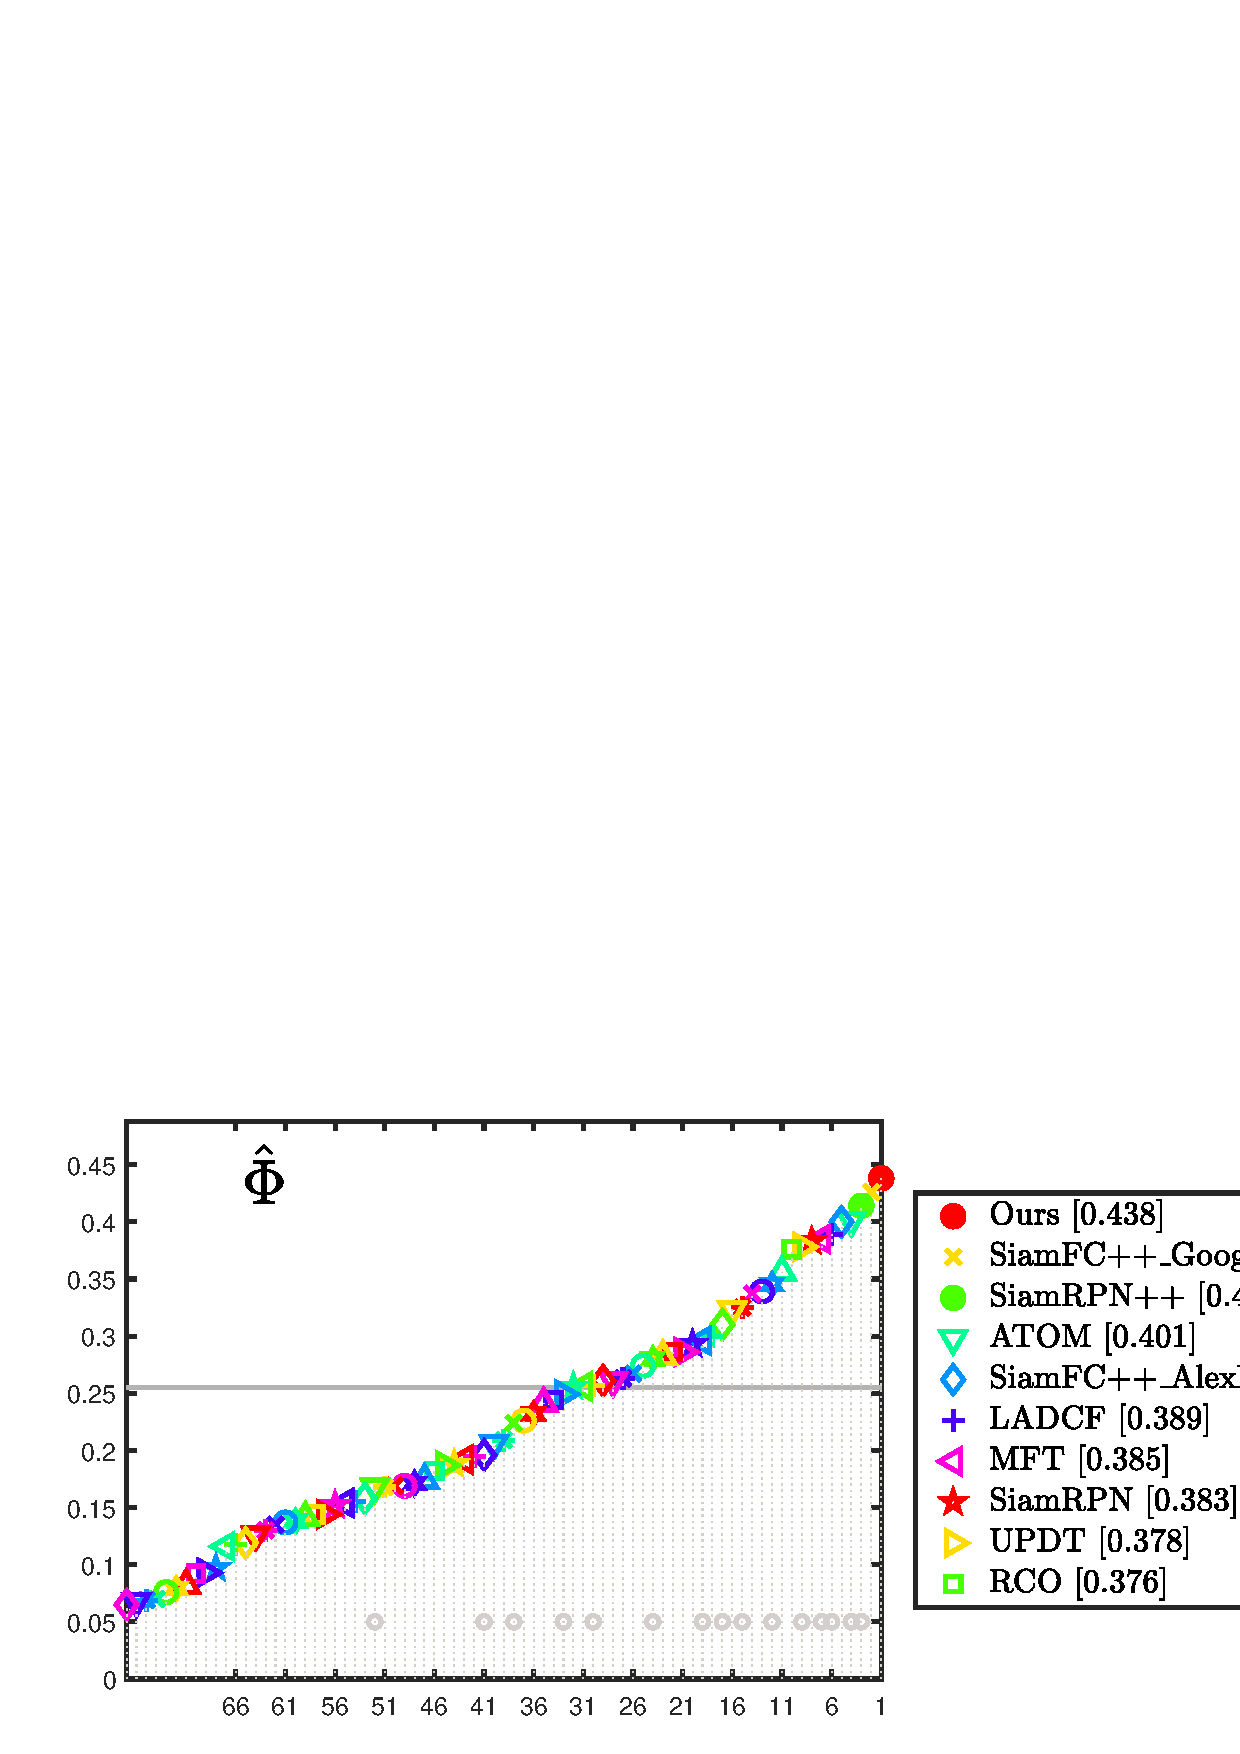
\includegraphics[width=0.48\textwidth]{Img/MTP/vot18/vot18_eao.png}
    \caption{Expected average overlap graph with trackers ranked from right to left. The right-most tracker is the top-performing according to the VOT2018 expected average overlap values.}
    \label{fig:eao}
\end{figure}
%%%%%%%%%%%%

%%%%%%%%%%%%%%%%%%%%%%%%%%%%%%%%%%%
\subsection{Implementation Details}
We use SiamFC++ \cite{SiamFC++} as our base tracker, and the backbone Siamese network adopts GoogLeNet \cite{szegedy2015going}. We do not perform any changes except for the model adaptation component. The parameter $\alpha$ in Equ. (\ref{equ:adaptaion}) is set to 0.05. Our method is implemented in Python with PyTorch. The proposed tracker runs at over 80 FPS on an NVIDIA RTX 2080Ti GPU.

%%%%%%%%%%%%%%%%%%%%%%%%%%%%%%%%%%%%%
\subsection{State-of-the-art Comparison}
\textbf{OTB2015} We use success rate to evaluate the performance of trackers on the OTB2015 dataset. Success rate relies on the intersection over union (IOU) of the predicted bounding box and the ground truth bounding box. We compare our method with various tracking algorithms, including ECO \cite{danelljan2017eco}, MDNet \cite{nam2016learning}, SiamRPN++ \cite{li2019siamrpn++}, ATOM \cite{danelljan2019atom} and SiamFC++\_GoogLeNet \cite{SiamFC++}. The iteration number for template update is set to 16. The results are shown in Table \ref{table:otb}. Our tracker outperforms the online tracker ATOM by 2.8\% in terms of the success score, which demonstrates the powerful model adaptation capability of our method.

\textbf{VOT2018} We compare our method with RCO \cite{kristan2018sixth}, UPDT \cite{bhat2018unveiling}, SiamRPN \cite{li2018high}, MFT \cite{kristan2018sixth}, LADCF \cite{kristan2018sixth}, ATOM \cite{danelljan2019atom}, SiamRPN++ \cite{li2019siamrpn++}, SiamFC++\_AlexNet \cite{SiamFC++} and SiamFC++\_GoogLeNet \cite{SiamFC++} on VOT2018. The trackers are compared using the robustness and accuracy measures. Robustness indicates the number of tracking failures, while accuracy denotes the average overlap between tracker prediction and the ground-truth box. Both of the measures are combined into a single expected average overlap (EAO) score. The iteration number for template update is set to 2. As shown in Fig. \ref{fig:eao}, the performances of all the listed trackers are not as good as our algorithm.

\textbf{GOT-10k} We use the average overlap (AO) score as performance measure following \cite{huang2018got}. We compare our method with CF2 \cite{CF2}, ECO \cite{danelljan2017eco}, CCOT \cite{CCOT}, GOTURN \cite{held2016learning}, SiamFC \cite{bertinetto2016fully}, SiamFCv2 \cite{valmadre2017end}, ATOM \cite{danelljan2019atom}, SiamFC++\_AlexNet \cite{SiamFC++} and SiamFC++\_GoogLeNet \cite{SiamFC++} on this dataset. The iteration number for template update is set to 2. In Fig. \ref{fig:got10k}, we can find that the proposed algorithm achieves better tracking performance compared with the listed state-of-the-art trackers.

\textbf{TrackingNet} We compare our method with SiamFC \cite{bertinetto2016fully}, ECO \cite{danelljan2017eco}, MDNet \cite{nam2016learning}, SiamRPN++ \cite{li2019siamrpn++}, ATOM \cite{danelljan2019atom}, SiamFC++\_AlexNet \cite{SiamFC++} and SiamFC++\_GoogLeNet \cite{SiamFC++}. The iteration number for template update is set to 32. Table \ref{tabel:trackingnet} shows that our tracker performs best in terms of precision and the normalized precision while maintaining a very competitive success value.

%%%%%%%%%%%%%%%%%%%%%%%%%%%
\subsection{Ablation Study}

%%%%%%%%%%%%%%%
\begin{table}[t]
\renewcommand\arraystretch{0.7}
\centering
\caption{Performance on OTB2015 using noisy initial frames.}
\begin{tabular}{c c c | c c}
\toprule
\multicolumn{3}{c|}{Coefficients of Noise} & \multicolumn{2}{c}{Success Score} \\
\midrule
$\gamma_1$ & $\gamma_2$ & $\gamma_3$  & SiamFC++\_G & Ours  \\
\midrule
0.57  &	1.6	 & 0.93	& 67.3    & 69.5 \\
%0.82  & 1.1  & 0.82 & 65.9    & 67.2 \\
0.88  & 0.22 & 0.86 & 65.7    & 68.0 \\
0.88  & 0.43 & 0.77 & 64.1    & 64.4 \\
0.92  & 0.98 & 0.82 & 65.6    & 66.6 \\
0.98  & 0.83 & 0.84 & 66.5    & 67.9 \\
1.0   & 0.81 & 0.79 & 65.3    & 66.0 \\
1.1   &	1.9  & 0.90	& 67.6    & 68.8 \\
1.2   & 0.70 & 0.79 & 65.7    & 66.6 \\
%1.3   & 1.3  & 0.77 & 64.9    & 65.8 \\
1.5   & 0.19 & 0.79 & 64.8    & 66.3 \\
%1.5   & 1.3  & 0.86 & 66.7    & 68.0 \\
\bottomrule
\end{tabular}
\label{table:noise}
\end{table}
%%%%%%%%%%%

%%%%%%%%%%%%%%%%
\begin{table}[t]
\renewcommand\arraystretch{0.8}
\centering
\setlength{\tabcolsep}{2pt}
\caption{11 attributes comparison on OTB2015 in term of success score.}
\begin{tabular}{r c c c c c c c c c c c}
\toprule
            & BC & DEF & FM            & IV            & IPR           & LR    & MB    & OCC   & OPR   & OV    & SV    \\
\midrule
SiamFC++\_G  &  62.5 & 63.9 & 68.0          & 69.2          & 69.5          & \textbf{72.5}  & 66.7 & 60.9 & 66.9 & 55.8 & 68.4 \\
Ours        & \textbf{66.5} & \textbf{66.8} & \textbf{68.7} & \textbf{71.3} & \textbf{69.6} & 69.8  & \textbf{67.3} & \textbf{62.5} & \textbf{68.4} & \textbf{57.1} & \textbf{69.8} \\
\bottomrule
\end{tabular}
\label{table:attr}
\end{table}
%%%%%%%%%%%

\iffalse
To verify the contribution of the proposed model adaptation method, we compare our tracker with the baseline SiamFC++\_GoogLeNet \cite{SiamFC++} on 4 challenging tracking datasets. In comparison with the baseline tracker on OTB2015, our tracker improves the success score by 1.4\%. On VOT2018, our tracker outperforms the baseline tracker by 1.2\% in terms of EAO. On GOT-10k, our tracker improves the AO score by 1.0\%. On TrackingNet, our tracker outperforms the baseline tracker by 1.7\% in terms of the normalized precision score. All these consistent improvements highlight the effectiveness of the proposed model adaptation method.
\fi

\textbf{Robustness to Noisy Initial Frames} To study how robust the approach is if the first frame is noisy compared to the next frames in the sequence, we add three kinds of noise to the first frame by: changing the image brightness, applying Gaussian blur, and using non-accurate ground truth bounding box annotation. We denote $\gamma_1 \in [0.5, 1.5]$ as the coefficient of brightness variation, $\gamma_2 \in [0, 2]$ the blur radius, and $\gamma_3 \in [0.75, 1]$ the IoU between the non-accurate first frame bounding box annotation and the real bounding box annotation, respectively. We run both the baseline tracker and our tracker 10 times on OTB2015 with randomly sampled $\gamma_1, \gamma_2$ and $\gamma_3$ (see Table \ref{table:noise}). Compared with SiamFC++\_GoogLeNet \cite{SiamFC++}, our tracker always performs better under different noise levels, which shows the robustness of our tracker to noisy initial frames.%the first frame noise.

\textbf{Attribute-based Analysis} For further analyses on the tracking performance, we also demonstrate the advantages of our algorithm through the attribute-based comparison on sequences of the OTB-2015 dataset (see Table \ref{table:attr}). In OTB2015, each sequence is annotated with 11 different attributes, namely: background clutters (BC), deformation (DEF), fast motion (FM), illumination variation (IV), in-plane rotation (IPR), low resolution (LR), motion blur (MB), occlusion (OCC), out-of-plane rotation (OPR), out-of-view (OV) and scale variation (SV). Compared with SiamFC++\_GoogLeNet \cite{SiamFC++}, our tracker achieves better performance on 10 out of 11 attributes, which demonstrates its robustness in challenging tracking scenarios such as illumination variation and motion blur.

%%%%%%%%%%%%%%%%%%%%
\section{Conclusion}
In this letter, we propose a novel model adaptation method for Siamese trackers, achieving accurate tracking with high speed. We show that the challenging model adaptation task in visual object tracking can be handled by simply manipulating pixels of the template image using the target ground-truth in the first frame. Our model adaptation method is pluggable, in the sense that it does not alter the overall architecture of the base tracker. Numerous experimental results on four object tracking benchmarks demonstrate the effectiveness of the proposed model adaptation method.